\chapter{Educational data minig}\label{chap1}
\minitoc
\thispagestyle{empty}
\newpage	
	
\section{Introduction}
Du fait que les systèmes informatisés conservent des journaux détaillés comme ceux des interactions utilisateur-système, ces journaux détaillés qui sont généralement dans une grande base de données ouvrent de nouvelles opportunités pour étudier ces données récolter. L’EDM est un domaine qui emprunte et étend des domaines connexes tels que l’apprentissage automatique (l’étude des programmes informatiques qui apprennent et s’améliorent avec des données empiriques), l’exploration du texte (approches pour trouver des modèles dans du texte), la psychométrie (l’étude des instruments psychologiques pour mesurer les compétences et les traits humains) et l’analyse des journaux Web (approches pour identifier les profils d’utilisateurs et la navigation modèles d’utilisateurs du site Web). Dans ce chapitre, nous présentons les techniques d’exploration de données, et un ensemble de technique d’analyse pour une variété de problèmes dans la recherche en éducation.\\

\section{Data mining}

\subsection{Définition}
L'exploration de données est un processus itératif et interactif visant à découvrir des modèles de données efficaces, nouveaux, utiles et compréhensibles dans de grandes bases de données. L'exploration de données, également appelée découverte de connaissances dans une base de données, fait référence à l'extraction de connaissances à partir de grandes quantités de données. Elle est utilisée pour extraire dans des grands volumes de données, des modèles cachés et des relations utiles dans la prise de décision. Bien que l'exploration de données et la découverte de connaissances de base de données soient souvent traitées comme des synonymes, elles font en fait partie du processus de découverte des connaissances. La séquence des étapes identifiées lors de l'extraction des connaissances à partir des données est illustrée à la figure \ref{extraction_connaissances} \cite{data_mining_concepts_techniques}.  \\
L'exploration de données est un domaine interdisciplinaire utilisant à la fois des techniques d'apprentissage automatique, de reconnaissance de formes et l'utilisation de statistiques, de bases de données et de visualisation pour déterminer les façons d'utiliser l'extraction d'informations à partir de très grandes bases de données \cite{cabena1998discovering}.

\begin{figure}[H]
	\begin{center}
		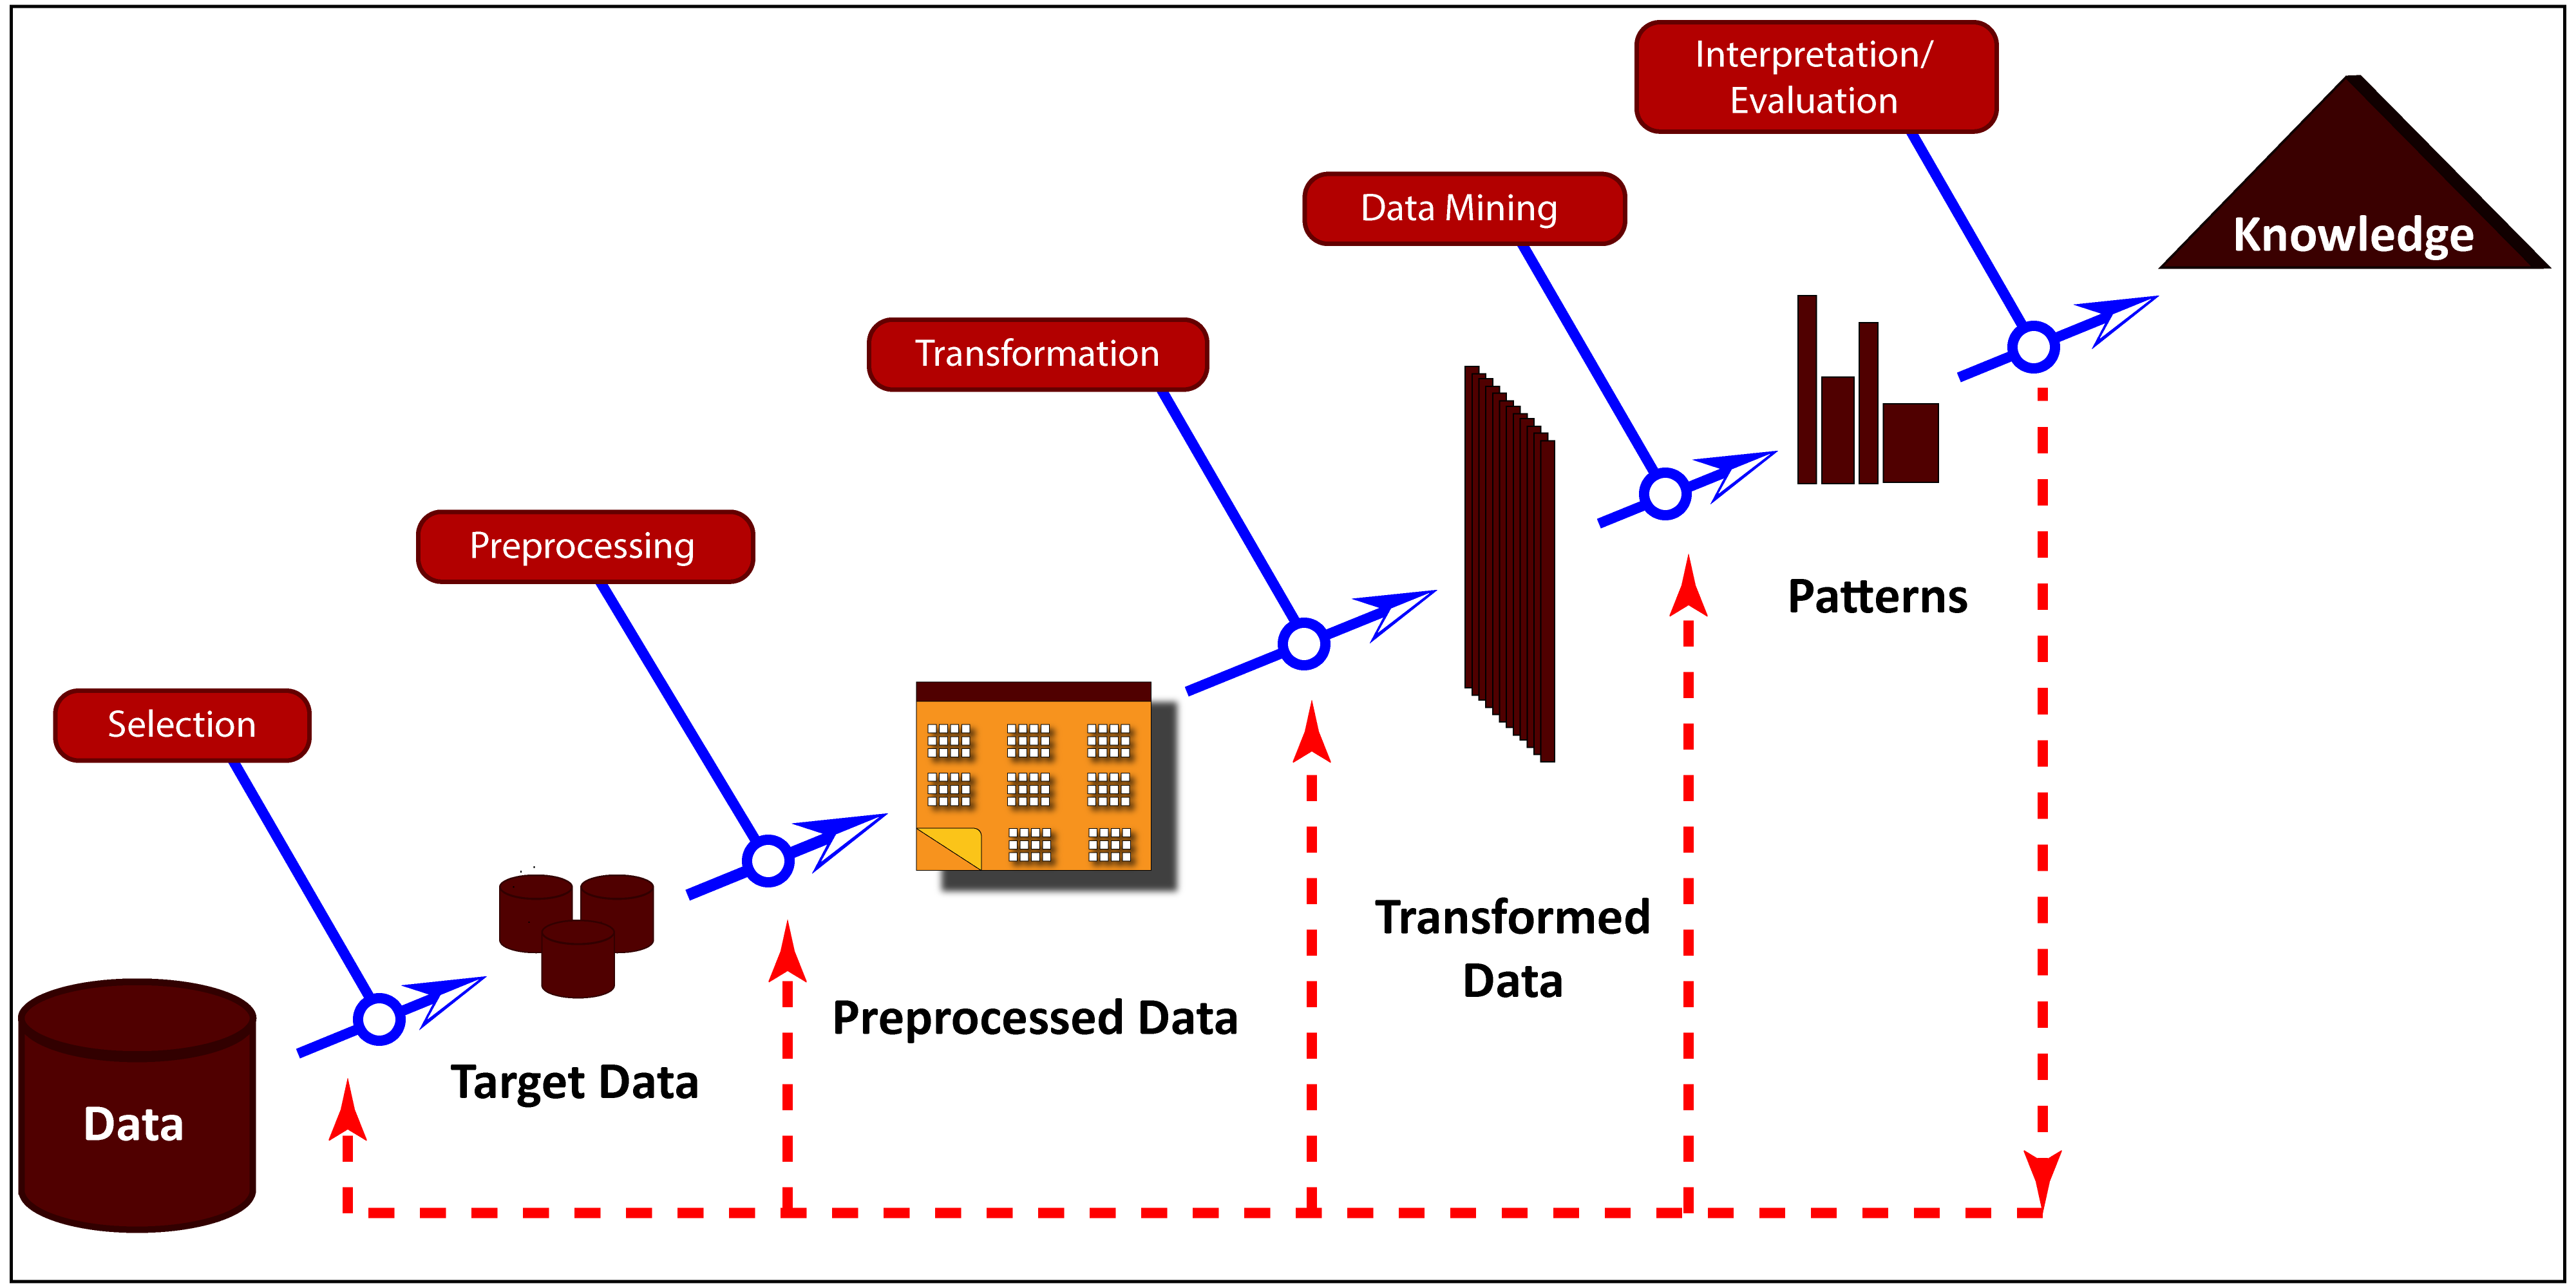
\includegraphics[width=\textwidth]{images/chapitre1/extract_data_steps.png}
	\end{center}
\caption{Les étapes de l'extraction de connaissances à partir de données}
\label{extraction_connaissances}
\end{figure}

\subsection{Les méthodes du data mining}
Le clustering et la classification sont deux tâches fondamentales dans l’exploration de données. La classification est principalement utilisée comme méthode d’apprentissage supervisé,
le clustering pour l’apprentissage non supervisé (certains modèles de clustering sont pour les deux). Le but du clustering est descriptif, celui de la classification est prédictif \cite{veyssieres1998identification}.« Comprendre notre monde nécessite de conceptualiser les similitudes et les différences entre les entités qui le composent » \cite{Educational_data_mining_a_survey_from_1995_to_2005}, de ce fait, certains coefficients de corrélations sont utilisés pour calculer la similarité entre deux éléments ou plusieurs et, des métriques et les critères de liaison permettent qu’en ta eux de déterminer le lien entre plusieurs entités afin de les groupées dans une même classe (c’est le cas du clustering). Certaines méthodes comme : « rule of association », « preaching », « neural networks », « decision trees » sont utilisé aussi pour explorer et analyser des jeux de données.


\section{Intelligent Tutorial Systems (ITS)}

\subsection{Définition}
Les systèmes de tutorat intelligents (ITS) sont des environnements d'apprentissage informatisés issus de l'IALT (Intelligent Computer Assisted Instruction) qui visent à personnaliser l'apprentissage. En effet, ils ont été développés pour répondre aux limites du CAI (Computer Assisted Instruction) en utilisant l'intelligence artificielle pour mettre en œuvre des systèmes plus flexibles et interactifs qui s'adaptent aux besoins spécifiques de l'apprenant en évaluant et en diagnostiquant ses problèmes afin de fournir les assistances \cite{buchecedric}. L'objectif est de mimer le comportement d'un tuteur humain en sa qualité de pédagogue expert et d'expert dans le domaine. Ainsi, tout comme un tuteur, un logiciel de ce type a le potentiel d'amener l'apprenant à accomplir une tâche et à fournir un retour sur leurs actions. ITS répond ainsi à la nécessité de placer l'apprenant au centre du processus d'apprentissage. \\
Les ITS sont essentiellement un environnement de résolution de problèmes ou d'exercice. Ils favorisent l'apprentissage dans un domaine spécifique en guidant et en aidant l'apprenant. Parfois, ils exposent d'abord le contenu de la matière à l’apprenant ; parfois ils présentent directement les exercices qui permettront à l'apprenant d'assimiler les connaissances \cite{handbook_of_educational_data_mining}.

\begin{figure}[H]
	\begin{center}
		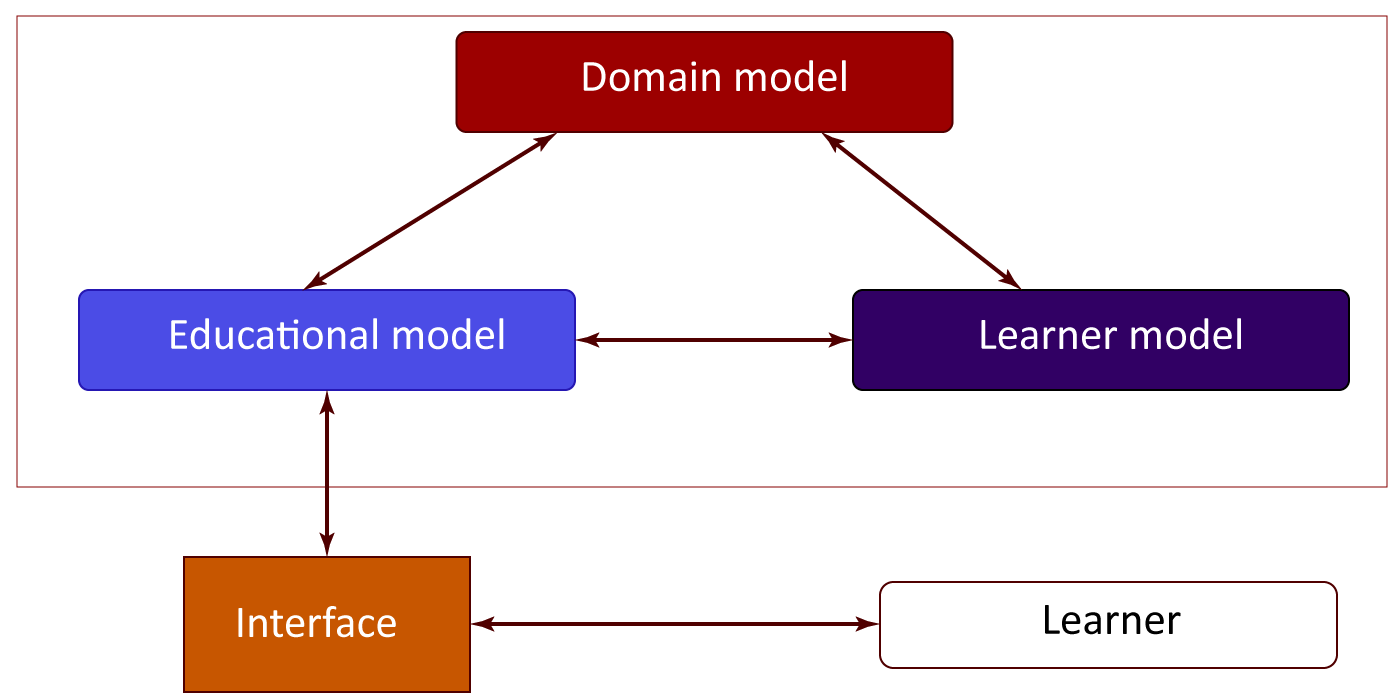
\includegraphics[width=\textwidth]{images/chapitre1/ITS architecture}
	\end{center}
\caption{L’architecture d’un ITS}
\label{itsArchitecture}
\end{figure}

\subsection{L’architecture d’un ITS}
L'architecture conceptuelle d'un ITS est illustrée à la figure \ref{itsArchitecture} et comprend : \cite{handbook_of_educational_data_mining}
\begin{itemize}
	\item[$\bullet$] \textbf{Un modèle d'interface :} qui représente la couche de communication entre l'apprenant et le système, c'est-à-dire les interactions entre l'apprenant et le système. Cette interface peut faire varier le type d'environnement d'apprentissage et l'objectif étant de privilégier une approche de conception qui ne gêne pas l'apprentissage. La qualité de l'interaction peut influencer les résultats d'apprentissage. Par conséquent, les principaux problèmes avec les interfaces d'apprentissage sont les problèmes d'interaction personne / machine. Pour surmonter ces problèmes, il faut prêter attention à la convivialité pour que la charge mentale associée à l’interface soit négligeable, ainsi qu’à l’utilité en facilitant l’accès, en permettant l’accès au domaine d’apprentissage et en soutenant la métacognition de l’apprenant. Les tendances actuelles s'orientent vers des dialogues tutoriels en langage naturel, l'intégration de la dimension affective dans l'interaction et les interfaces tangibles.	
	\item[$\bullet$] \textbf{Modèle du domaine :} également appelé modèle expert, il représente l'expertise de l'enseignant dans le domaine, c'est-à-dire ce qui doit être enseigné. L’expertise peut être modélisée de trois manières : une approche « boîte noire » : appliquer toute méthode de raisonnement sur le domaine inexpliqué, sans aucune transparence pour l'utilisateur ; un système expert peut expliquer son raisonnement et un modèle cognitif : simuler la manière dont les humains utilisent les connaissances.
  \item[$\bullet$] \textbf{Un modèle d'apprentissage :} qui peut personnaliser l'apprentissage en tenant compte des spécificités de l'apprenant.
  \item[$\bullet$] \textbf{Un modèle éducatif :} qui sait enseigner.
\end{itemize}
    
\section{Educational Data mining}
\subsection{Définition}
La communauté d'exploration de données appliquée dans l'éducation a défini ce terme comme suit : L'exploration de données appliquée dans l'éducation est une discipline qui concerne le développement de méthodes permettant d'explorer les types uniques de données provenant des milieux éducatifs. Ces méthodes sont utilisées pour mieux comprendre le comportement des apprenants et environnement de leur apprentissage \cite{state_of_educational_data_mining_in_2009_a_review_and_future_visions}. \\
L'exploration de données éducatives (EDM) vise à développer, rechercher et appliquer des méthodes informatisées pour détecter des modèles dans de grandes collections de données éducatives qui seraient autrement difficiles ou impossibles à analyser en raison de l'énorme volume de données dans lesquelles elles existent \cite{Educational_data_mining_a_survey_from_1995_to_2005}. \\
Ce domaine est une forme d'intersection des trois domaines principaux tels que : l'informatique, l'éducation et les statistiques illustrés dans la figure \ref{domaine_exploration_données}.

\begin{figure}[H]
	\begin{center}
		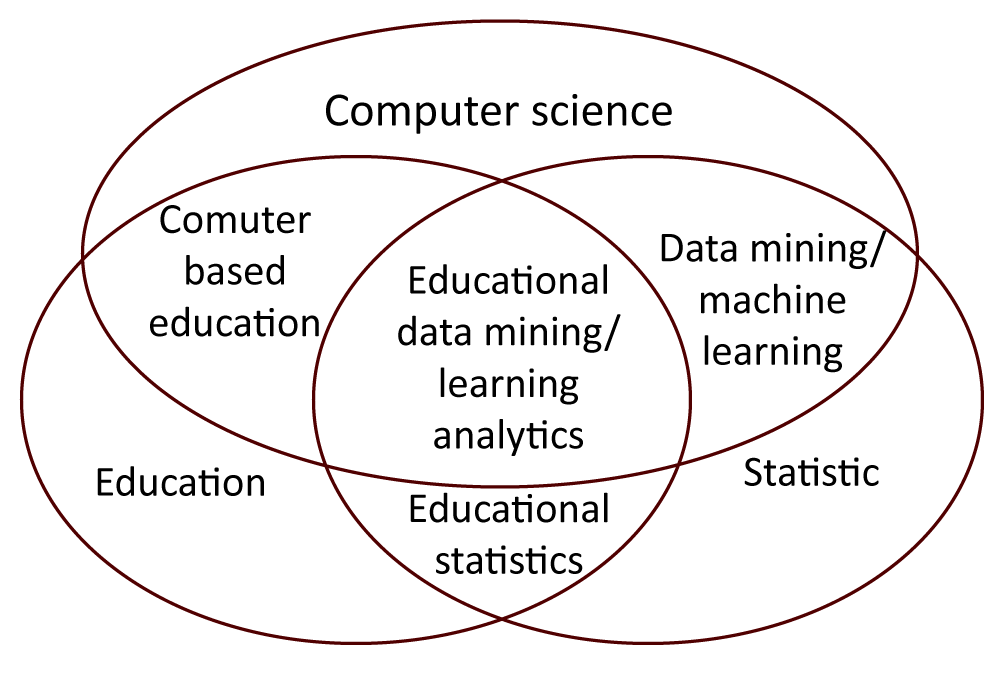
\includegraphics[scale=0.3]{images/chapitre1/Principaux domaines liés à l'exploration de données éducatives}
	\end{center}
  \caption{Principaux domaines liés à l'exploration de données éducatives}
  \label{domaine_exploration_données}
\end{figure}

Les techniques d'exploration de données (EDM) sont devenues plus importantes dans la recherche et le développement en raison du développement rapide de la technologie, de la croissance rapide des connaissances humaines et de l'augmentation du nombre de personnes détenant des systèmes d'enseignement informatisé. \\
    
\subsection{Processus d'application du DM en éducation}
Le processus d'application de l'exploration de données appliqué dans l'éducation peut être considéré comme un cycle itératif de formulation, de test et de raffinement d'hypothèses. Dans ce processus, l'objectif n'est pas seulement de transformer les données en connaissances, mais aussi de filtrer les connaissances extraites pour savoir comment les modifier. \\
L’environnement éducatif pour améliorer l’apprentissage des apprenants est présenté dans la figure \ref{dataMiningProcess}. Des études ont montré que l'application de l'EDM est similaire au processus Knowledge from Data (KDD). Ce processus commence par la collecte de données à utiliser à partir de l'environnement éducatif. \\
Les données brutes obtenues nécessitent un nettoyage et un prétraitement tels que : fusion de données hétérogènes, traitement des données manquantes, conversion de données d'une source de données à une autre, et données, etc. Cette phase nécessite souvent l'utilisation de certaines données techniques minières. Le résultat de ce dernier est un modèle capable de structurer les données stockées. Enfin, la dernière étape est l'interprétation et l'évaluation des résultats obtenus \cite{dm_tuteurs}.

\begin{figure}[H]
	\begin{center}
		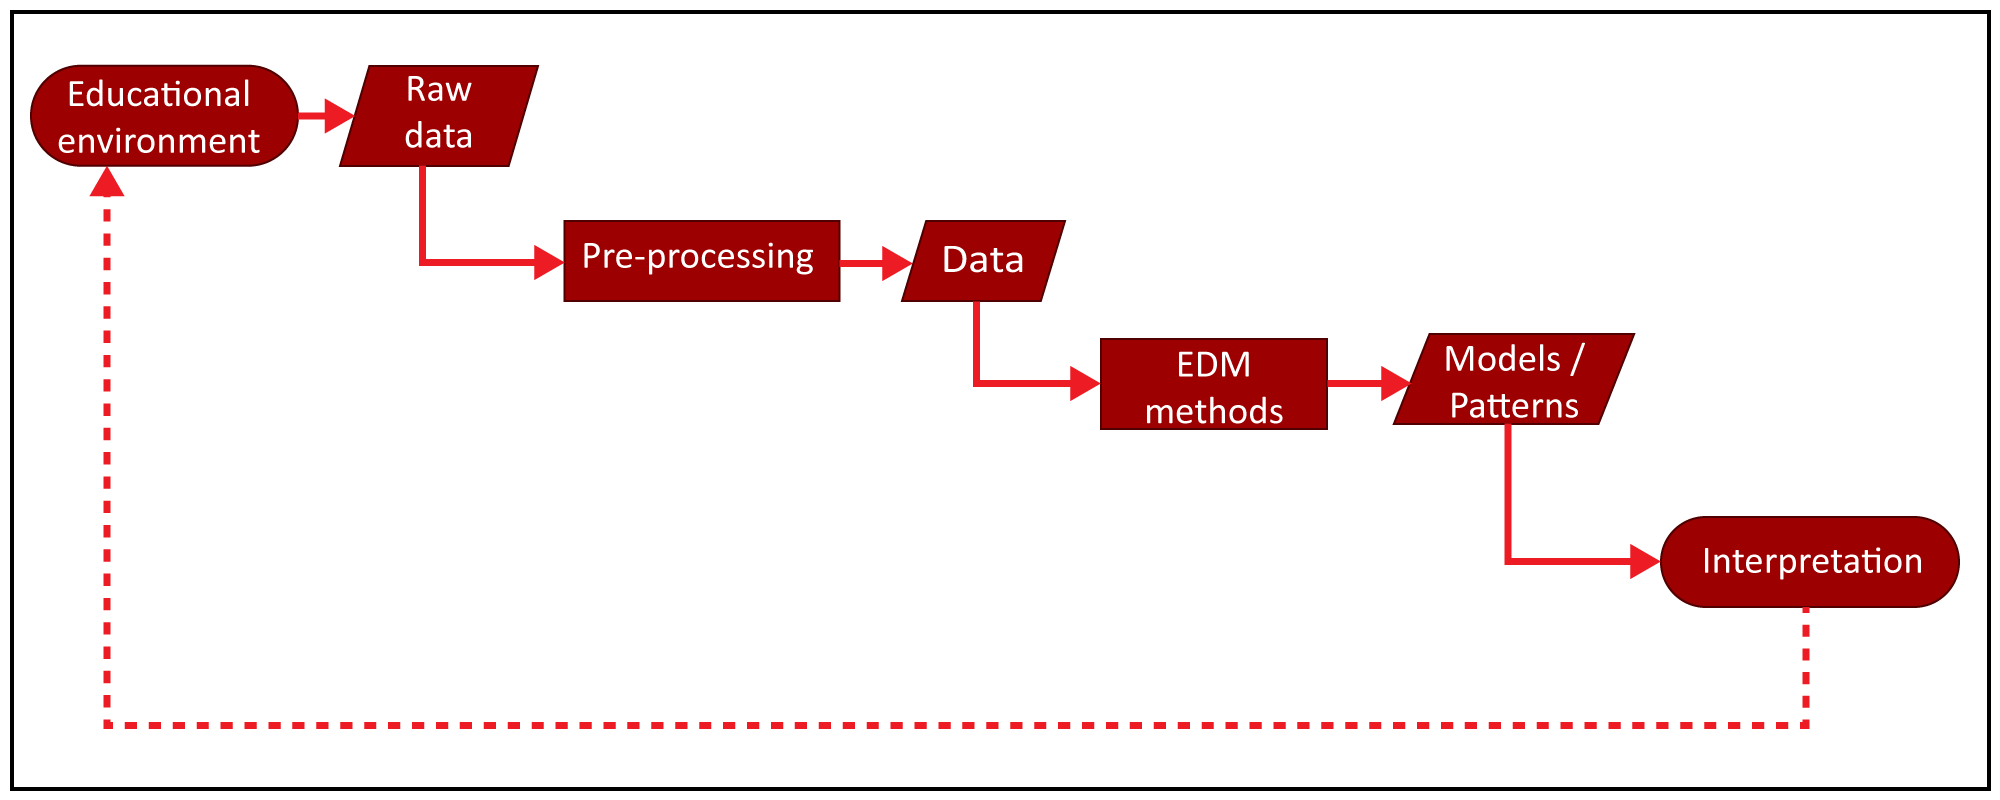
\includegraphics[width=\textwidth]{images/chapitre1/Data mining application process applied in education}
	\end{center}
\caption{Data mining application process applied in education}
\label{dataMiningProcess}
\end{figure}

\subsubsection{Les méthodes d’analyse et d’exploration appliquer dans EDM}
Certaines méthodes du data mining ont été largement appliquées sur les données issues des systèmes éducatifs afin d’obtenir des connaissances cacher et des modèles. Les méthodes du data mining ont été appliquer dans plusieurs domaines de recherche tels que : le e-learning, le système de tuteur intelligent, text mining, réseaux sociaux, web mining, etc. Les méthodes d’analyse et d'exploration de données éducatives sont tirées de diverses sources littéraires, notamment l'apprentissage automatique, la psychométrie et d'autres domaines de la modélisation information, des statistiques et de la visualisation de l'information. \\

\begin{figure}[H]
	\begin{center}
		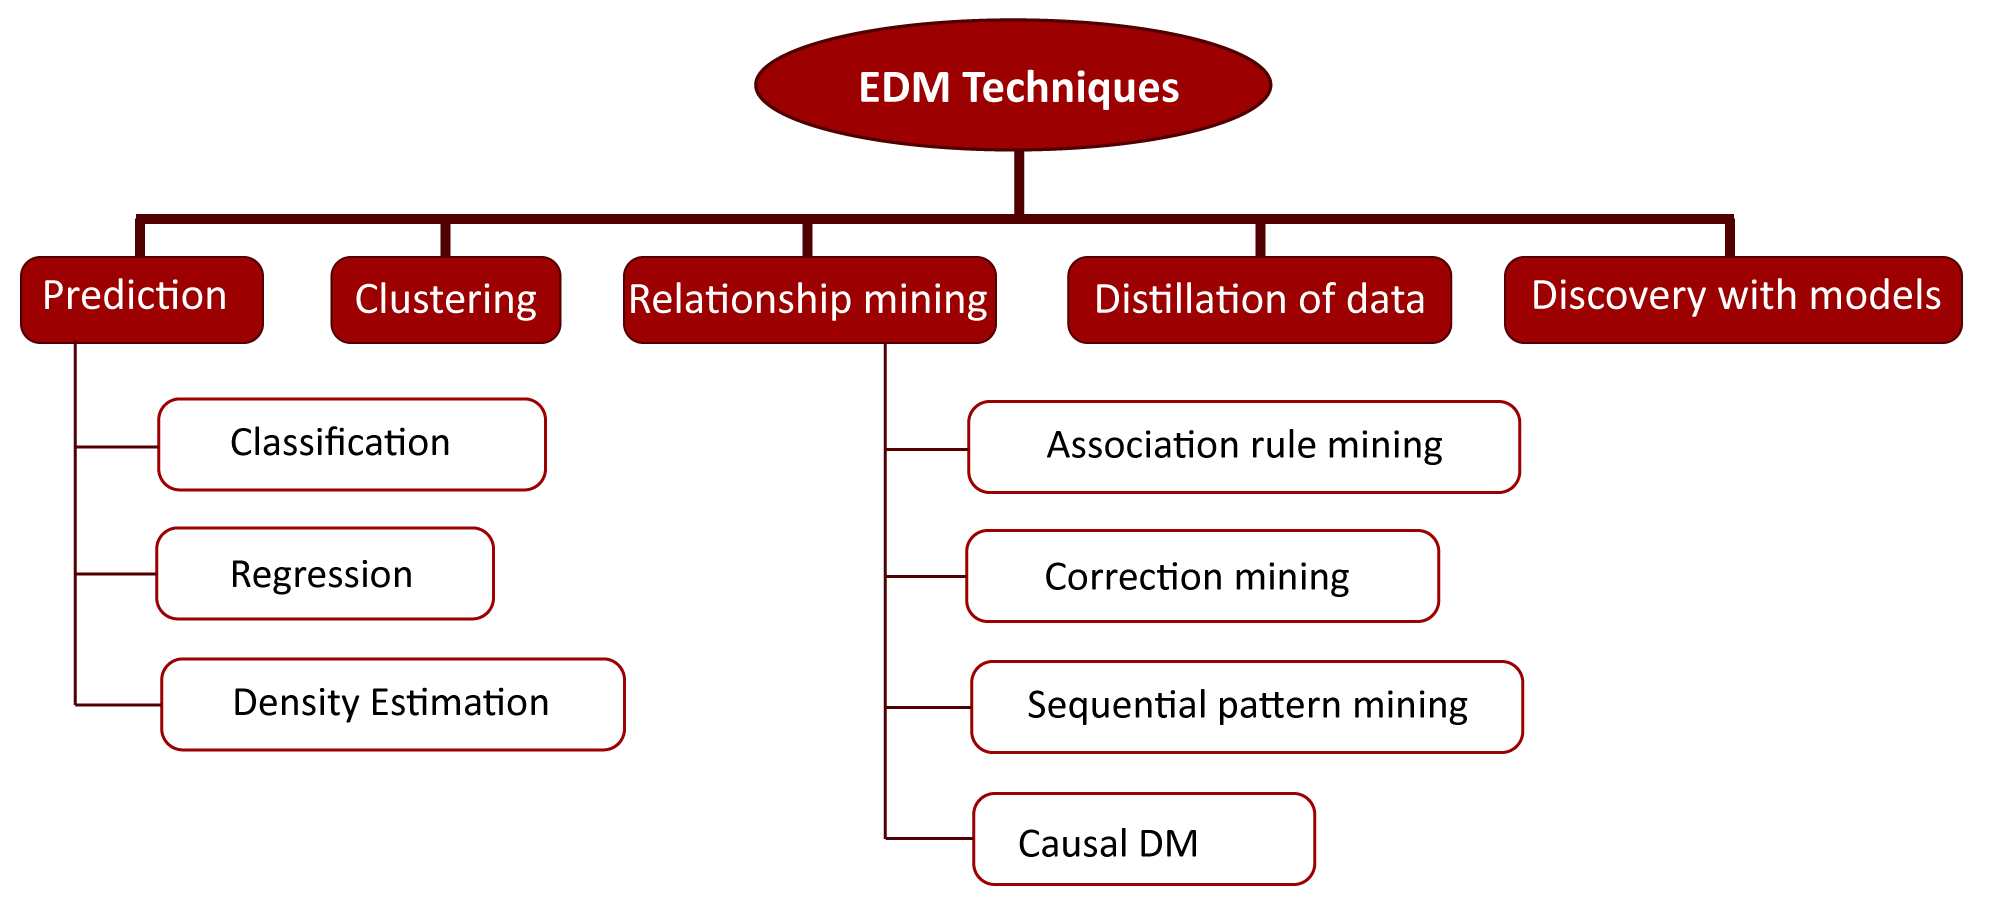
\includegraphics[width=\textwidth]{images/chapitre1/edm techniques}
	\end{center}
	\caption{Les techniques d'exploration de données éducatives.}
\end{figure}

\paragraph{Modèle supervisée \\}

L'induction de modèle supervisée comprend des techniques d'apprentissage automatique qui déduisent des modèles de prédiction à partir de instances d'entraînement pour lesquelles les valeurs d'un attribut cible sont connues. Les modèles de prédiction acceptent des
instances en entrée (généralement décrites comme un vecteur d'attribut) et en sortie une prédiction pour la variable cible. Les modèles qui prédisent des valeurs cibles catégorielles sont appelés modèles de classification ; des modèles qui prédire les valeurs cibles continues sont appelés modèles de régression. Les modèles de prédiction peuvent être basés sur
différentes représentations, par exemple, les arbres de décision, les machines à vecteurs de support et modèle de régression linéaire \cite{Scheuer2012}.

\paragraph{Modèle non supervisée \\}

L'induction de modèle non supervisée comprend des techniques d'apprentissage automatique qui déduisent des modèles à partir d'instances d'apprentissage pour lesquelles les valeurs d'un attribut cible ne sont pas connues. 
Les méthodes non supervisées utilisent une approche ascendante, c'est-à-dire que les modèles et les structures 
sont recherchés dans l'espace d'entrée sans catégories cibles explicitement définies ni exemples étiquetés. 
Une approche largement utilisée est le clustering, qui est utilisé pour identifier des groupes d'instances dans 
un ensemble d'apprentissage qui sont « similaires » à certains égards. En règle générale, une sorte de mesure de 
distance (par exemple, la distance euclidienne) est utilisée pour décider de la similitude des instances. Une fois un 
ensemble de clusters a été déterminé, de nouvelles instances peuvent être classées en déterminant le cluster le plus 
proche. Un algorithme de clustering bien connu est le clustering k-means \cite{Scheuer2012}.
    
\paragraph{L'estimation des paramètres \\}
L'estimation des paramètres comprend des techniques statistiques pour déduire des paramètres de modèles probabilistes à partir d’un jeu de données. Ces modèles peuvent être utilisés pour prédire la probabilité d'événements d'intérêt. L'approche est basée sur l'hypothèse que le modèle a une forme paramétrique donnée (par exemple, une distribution gaussienne avec les paramètres moyenne et variance). Un exemple d'application en EDM est l'estimation des paramètres Bayesian Knowledge Tracing (BKT). Le BKT est utilisé pour déterminer la probabilité qu'un élève maîtrise une compétence sur la base de l'historique des performances passées. Un modèle BKT peut être compris comme un réseau bayésien dynamique avec quatre paramètres (priorité, estimation, glissement et taux d'apprentissage). Ces paramètres peuvent être déterminés, par exemple, avec l'algorithme Espérance-Maximisation \cite{Scheuer2012}. Aussi l’utilisation de la théorie des réponses aux items (Item Response Theory IRT) permet de capter plus de nuances dans le comportement humais et d’estimer la capacité de l’apprenant à réussir un item et aussi d’estimer la difficulté, la discrimination des items.

\paragraph{L'exploration de relations (Relationship mining) \\}
L'exploration de relations concerne l'identification des relations entre les variables, des relations qui peuvent être de nature associative, corrélationnelle, séquentielle ou causale. Par exemple, une approche courante de l'exploration de règles d'association consiste à apprendre les règles SI-ALORS qui dépassent un seuil minimum de « support » et de « confiance ». La prise en charge indique la fréquence relative des transactions qui correspondent à la fois aux parties IF et ALORS de la règle. La confiance dénote la fréquence relative des transactions qui correspondent à la partie THEN de la règle dans l'ensemble de transactions qui correspondent à la partie IF. Apriori est, par exemple, un algorithme de règle d'association classique. Un exemple d'application en EDM est l'identification d'erreurs qui se produisent fréquemment ensemble (par exemple, les étudiants qui ont commis les erreurs A et B ont également souvent commis l'erreur C) \cite{Scheuer2012}.

\paragraph{La distillation des données pour le jugement humain (Distillation of data for human judgment) \\}
La distillation des données pour le jugement humain vise à représenter les données de manière intelligible à l'aide de statistiques, méthodes de visualisation et interfaces d'information interactives. Par exemple, les performances moyennes les scores peuvent être calculés pour chaque élève et présentés à un enseignant par ordre croissant dans un graphique à barres. Un autre exemple est les courbes d'apprentissage, qui tracent les performances d'un élève (par exemple, le temps de réponse) par rapport au nombre d'occasions de pratiquer une compétence. Une courbe d'apprentissage idéale montre que la performance s'améliore en douceur et de façon monotone, suivant approximativement une loi de puissance ou une fonction exponentielle. D'un autre côté, les courbes d'apprentissage avec des pointes indiquent qu'une autre compétence pourrait interférer avec la compétence réellement modélisée, c'est-à-dire que le modèle de compétence pourrait être amélioré \cite{Scheuer2012}.

\paragraph{Discovery with models \\}
Discovery with models (découverte avec des modèles) comprend des approches qui amorcent des modèles déjà existants pour faire des découvertes plutôt que de calculer de nouveaux modèles à partir de zéro. Par exemple, un modèle de prédiction pourrait être appliqué à un ensemble de données pour prédire les valeurs d'une catégorie cible d'intérêt. Les prédictions elles-mêmes pourraient être utilisés à nouveau comme données dans d'autres analyses, par exemple, ils pourraient être corrélés avec une catégorie cible d’un autre modèle de prédiction. Un autre exemple consiste à scruter les différentes composantes d'un modèle de prédiction pour en savoir plus sur les facteurs qui influencent la prédiction \cite{Scheuer2012}.

\section{Conclusion}
Dans ce chapitre, nous avons passé en revue le domaine de l'exploration de données éducatives, en présentant brièvement ses applications et ses techniques. L'application des méthodes d'exploration de données dans le secteur de l'éducation est un phénomène intéressant. Les techniques d'exploration de données dans les organisations éducatives nous aident à apprendre davantage sur les performances des apprenants, le comportement des apprenants, la conception des programmes et à motiver les apprenants sur divers paramètres.
	
	